\subsubsection{Multithread}
\label{subsec:logstashmultithread}
{\footnotesize Attention ces informations sont pour le moment, \textit{Jeudi 16 Avril 2015}, correctes 
mais sont amenées à changer, notamment concernant les outputs.}

Chaque plugin input utilise un \gls{thread}. Cela permet d'éviter les engorgements si  
certaines entrées sont plus longues à traiter que d'autres.

Le bloc filtre entier utilise, par défaut, un seul thread. Mais, il est possible 
d'augmenter le nombre de threads affectés au traitement des filtres avec le \gls{flag}
-w lors du démarrage de Logstash.

À l'heure actuelle, le bloc output de logstash ne peut utiliser qu'un seul thread.
Il lit donc sa queue de façon séquentielle. 

\subsection{Moteur d'expression régulière}
\label{subsec:logstashregexengine}
Les expressions régulières utilisées par Logstash dans le plugin grok utilisent le 
moteur Oniguruma dont les spécifications sont disponibles à cette 
\href{http://www.geocities.jp/kosako3/oniguruma/doc/RE.txt}{adresse}\footnote{http://www.geocities.jp/kosako3/oniguruma/doc/RE.txt, 
si des symboles \textbf{ \textyen} apparaissent vous avez probablement un problème d'UTF8 sur 
votre navigateur, ils correspondent à des \textbf{ \textbackslash}}.
Ruby n'utilise plus Oniguruma depuis la version 2.0 mais son fork Onigmo\footnote{
dixit Wikipédia https://en.wikipedia.org/wiki/Oniguruma}. Mais cette évolution ne
s'applique pas à Logstash puisque ce dernier est codé en Jruby.

\subsection{Sense}
\label{subsec:elasticsense}
Ce module chrome a été développé par Boaz Leskes. Il sert de client à ElasticSearch
pour éviter d'avoir à le manipuler directement via curl.

Le développement (public) de ce module est arrêté depuis son intégration dans \emph{Marvel} 
le logiciel de monitoring et d'optimisation, vendu\footnote{voir basde page : 
\url{https://www.elastic.co/products/marvel/signup.html}} par la société \emph{elastic}.


\subsubsection{Installation}
Installer Sense est simple comme installer une extension 
Chrome\footnote{testé sur chromium} tierce.
Tout d'abord : récupérer le module à l'adresse \url{https://github.com/bleskes/sense}
en utilisant par exemple : 
\begin{lstlisting}[style=code,label=lst:gitclonesense]
git clone https://github.com/bleskes/sense.git
\end{lstlisting}

Il suffit ensuite de l'activer dans chromium :\\ 
chrome://extension => Developer mode => Load unpacked extension.
\begin{figure}[H]
\center
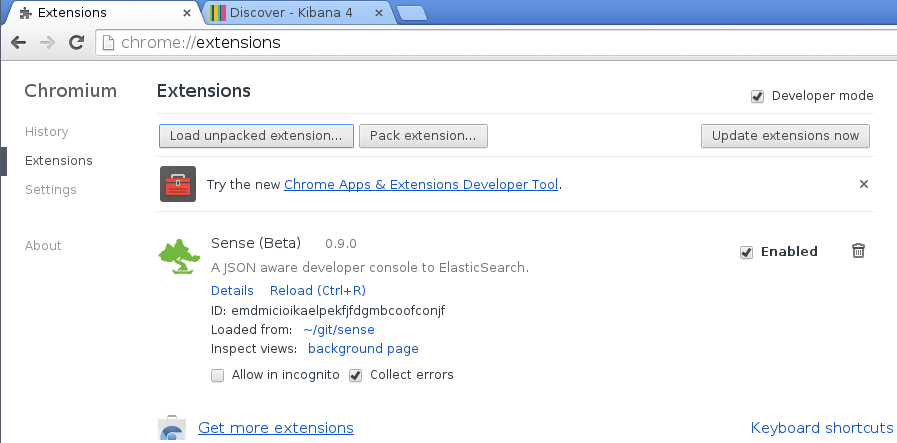
\includegraphics[width=12cm]{senseinstall.png}
\label{fig:senseinstall}
\caption{Plugin Sense installé dans chromium}
\end{figure}
Et voilà ! \footnotesize{(avec un accent anglais)}
\subsubsection{Utilisation de Sense}

\begin{figure}[H]
\center
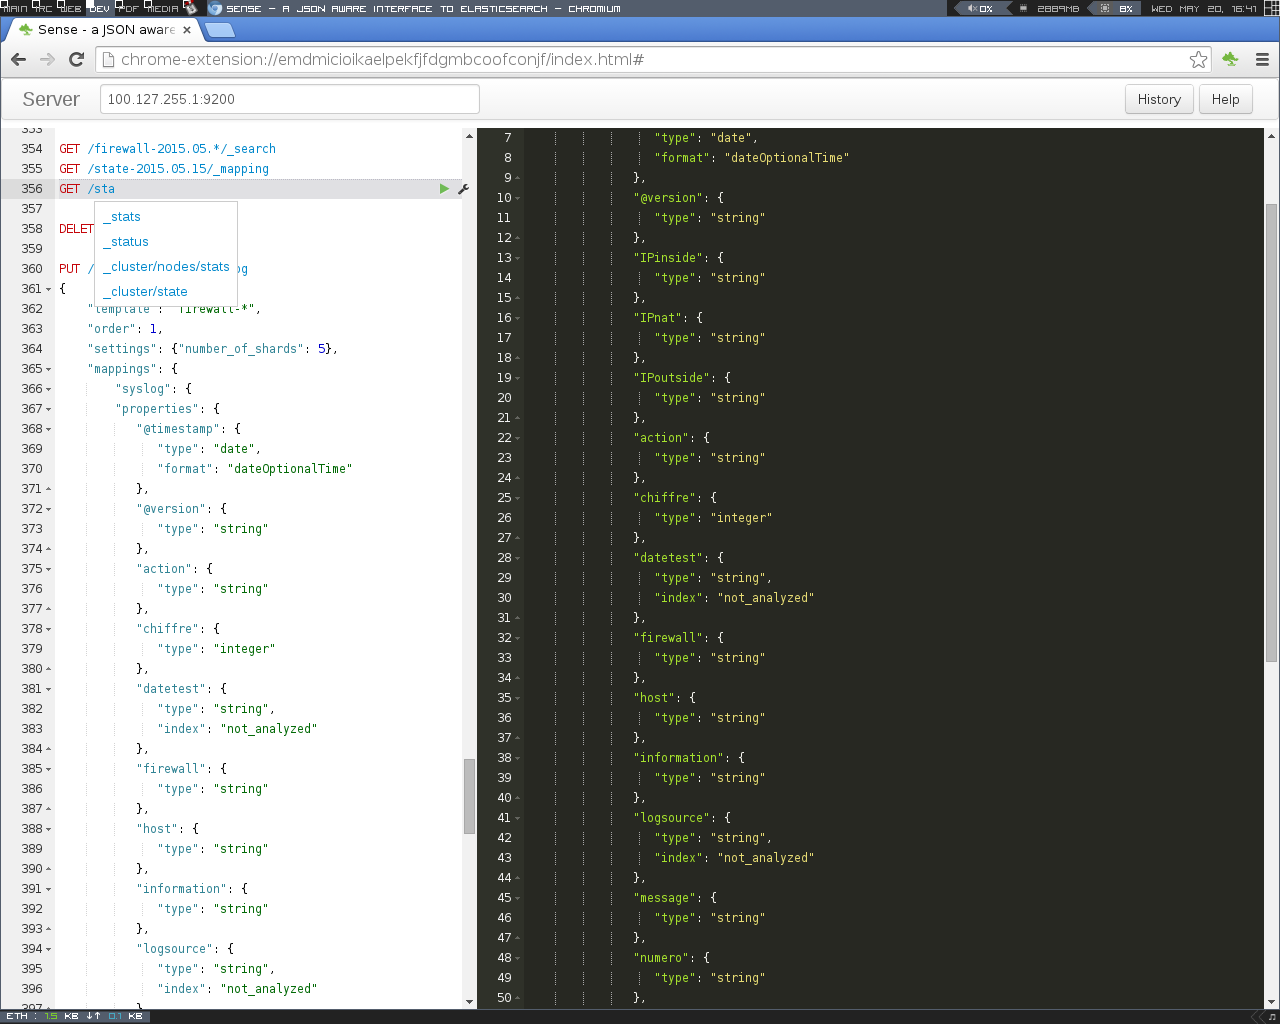
\includegraphics[width=1\textwidth]{sensegui.png}
\label{fig:sensegui}
\caption{Vue générale de Sense}
\end{figure}

Nous allons à l'aide de l'image ci-dessous brièvement expliquer le fonctionnement de Sense
\begin{figure}[H]
\center
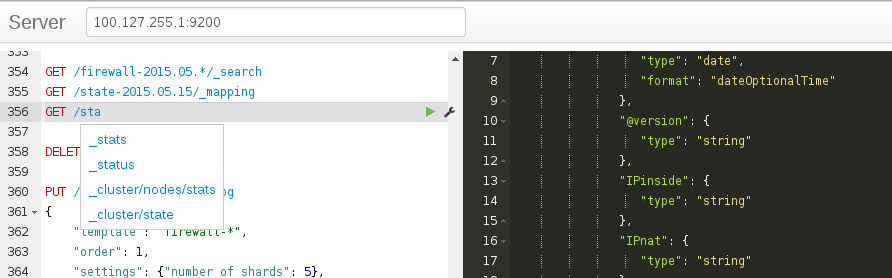
\includegraphics[width=15cm]{sensegui2.png}
\label{fig:sensegui2.png}
\caption{Zoom sur les fonctionnalités de Sense}
\end{figure}
Le formulaire \textbf{Server} situé en haut correspond à l'adresse et au port d'écoute 
de l'instance Elasticsearch sur laquelle on souhaite travailler.

Le panneau de gauche correspond au \textbf{panneau de requête}. On utilise l'API 
REST d'Elasticsearch pour envoyer des requêtes (recherches, modifications\ldots 
une présentation de l'API est réalisé ultérieurement). Il est à noté que le panneau 
de gauche est doté d'une autocomplétion pour les fonctions et les éléments standards 
d'Elasticsearch.

Le panneau de droite est le \textbf{panneau de réponse} aux requêtes. Les informations
nous parviennent en JSON.

\subsection{Full text}
\label{subsec:elasticfulltext}
Le full text s'oppose aux valeurs exacts.
Les champs non analysés sont traités comme des valeurs exacts.
Comme expliqué plus haut, les chiffres, les booléens, les dates, sont des valeurs 
exacts. Il est possible qu'une chaine de caractère en soit une aussi.

\textbf{"Le chien"} est différent de \textbf{"le chien"} ou encore de \textbf{"Lechien"}.

Pour le full text la notion d'index et d'analyseur est primordiale. L'analyseur va
décidé de comment les différents membres de la chaine de caractère vont être considérés.
Après cette étape ces membres vont être indexés et une recherche les renverra par 
popularité décroissante.

Puisqu'un exemple vaut mieux qu'un long discours, je vais m'inspiré de ceux donnés
dans \textit{"The Definitive guide to Elasticsearch"}.


Considérons 2 phrases :
\begin{itemize}
    \item The quick brown fox jumped over the lazy dog
    \item Quick brown foxes leap over lazy dogs in summer
\end{itemize}

\begin{figure}[H]
\center
\begin{tabular}{|l||c|c|}
\hline
\textbf{Termes}   & \textbf{P1}    & \textbf{P2}\\ \hline  
Quick   &       &  X\\ \hline  
The     &   X   &   \\ \hline
brown   &   X   &  X\\ \hline
dog     &   X   &   \\ \hline
dogs    &       &  X\\ \hline
fox     &   X   &   \\ \hline
foxes   &       &  X\\ \hline
in      &       &  X\\ \hline
jumped  &   X   &   \\ \hline
lazy    &   X   &  X\\ \hline
leap    &       &  X\\ \hline
over    &   X   &  X\\ \hline
quick   &   X   &   \\ \hline
summer  &       &  X\\ \hline
the     &   X   &  X\\ \hline 
\end{tabular}
\caption{Index des phrase}
\end{figure}
Lors d'une recherche full text, Elasticsearch va créer ce genre de listes.

Si je cherche \emph{quick brown}, le tableau ressemblerait à cela 


\begin{figure}[H]
\center
\begin{tabular}{|l||c|c|}
\hline
\textbf{Termes}   & \textbf{P1}    & \textbf{P2}\\ \hline  
brown   &   X   &  X\\ \hline
quick   &   X   &   \\ \hline \hline
Total   &   2   &  1 \\ \hline
\end{tabular}
\caption{Index correspondant à une recherche}
\end{figure}

On voit donc bien que la phrase la plus populaire est la phrase 1. On constate également
que Elasticsearch \emph{fait une différence entre \emph{Quick} et \emph{quick}}. 
Cela est est réglable (on peut, ne pas tenir compte de la casse).
Ce qu'il faut retenir c'est que pour discriminer efficacement, il est aussi possible
d'utiliser des syntaxe comme +fox, de même on peut faire une recherche avec un bloc
de deux termes pour être plus efficace : "over the" qui n'existe que dans P1.

\subsection{Settings}
\label{subsec:settings}
Si un doute s'était imissé dans notre esprit, les paramètres de Kibana, concernent
uniquement Kibana, et pas Elasticsearch,\hyperref[fig:kibanatuto14]{ certaines informations} 
sont cependant affichées pour aider l'utilisation de Kibana mais pas de possibilité 
de les modifier.

En revanche, il faut bien avouer que leurs consultations est plus agréable depuis 
Kibana que depuis l'export json d'Elasticsearch.

\begin{figure}[H]
\center
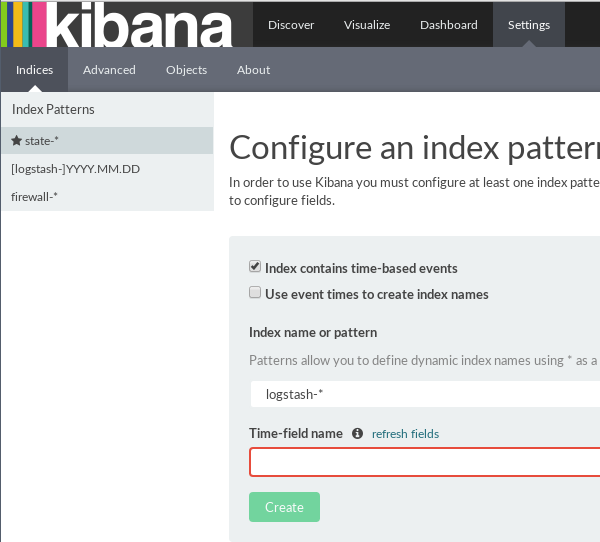
\includegraphics[width=1\textwidth]{kibanatuto/rap/20.png}
\label{fig:kibanatuto13}
\caption{Accueil de settings}
\end{figure}

Dans cette page vous pouvez créer de nouveaux ensembles d'index, ou en choisir un 
déjà existant.

En choisissant un index nous obtenons des informations sur son mapping, ce qui peut 
être utile pour effectuer des recherches plus pertinenentes.


\begin{figure}[H]
\center
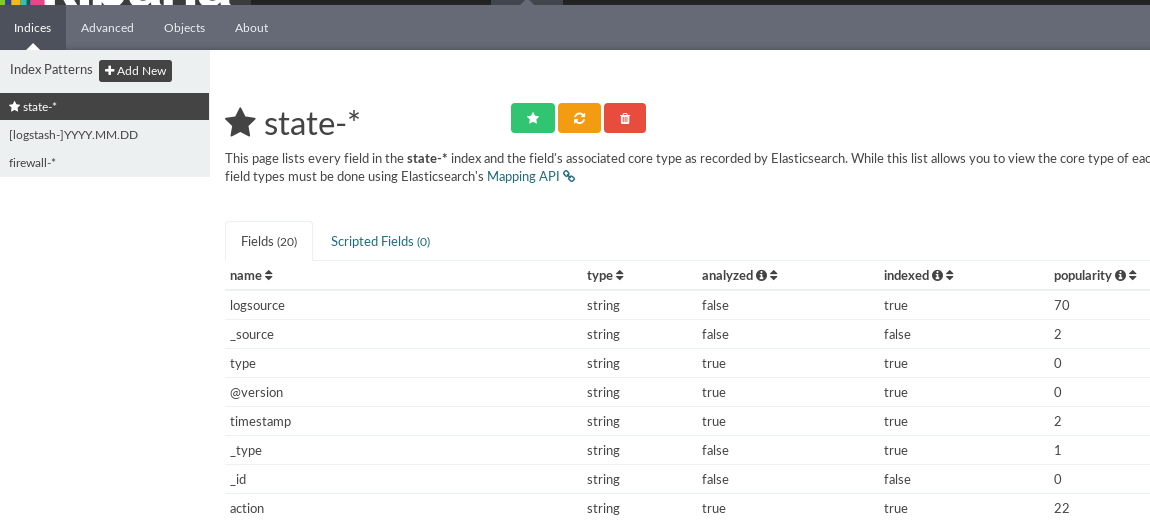
\includegraphics[width=1\textwidth]{kibanatuto/rap/22.png}
\label{fig:kibanatuto14}
\caption{Mapping d'un index}
\end{figure}

Enfin, c'est aussi dans cette section que l'on a une liste et que l'on peut supprimer les 
objets enregistrés (recherche, visualisations, dashboard)

\begin{figure}[H]
\center
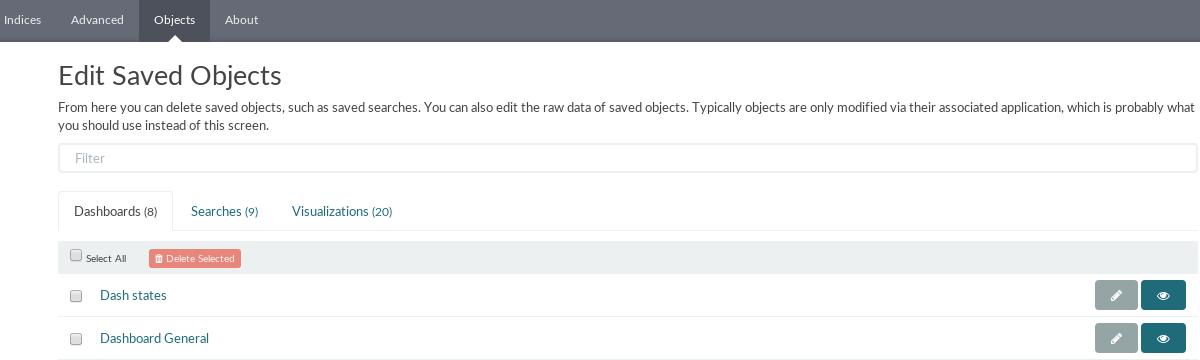
\includegraphics[width=1\textwidth]{kibanatuto/rap/23.png}
\label{fig:kibanatuto15}
\caption{Liste des objets}
\end{figure}

